\documentclass[a4paper]{article}
\usepackage[a4paper,left=2.5cm,right=2cm,top=2.5cm,bottom=2.5cm]{geometry}
\usepackage[italian]{babel}
\usepackage[T1]{fontenc}
\usepackage{graphicx} % per \includegraphics
\usepackage{amsmath} % senza si rompe il \text
%\usepackage{amssymb}
\usepackage{hyperref} % riferimenti alla bibliografia
\usepackage{booktabs} % per le tabelle
\usepackage{listings} % per i blocchi di codice
\usepackage{setspace} % per gli spazi nell'indice
\usepackage[backend=biber,sorting=none]{biblatex}
\addbibresource{bibliografia.bib}
\usepackage{xcolor}


\usepackage{scrextend} % per settare il font > 12pt
\changefontsizes[18pt]{14pt}

\usepackage{caption} % per le caption sotto le immagini
\captionsetup{figureposition=bottom,font=small}
\captionsetup{tableposition=top,font=small}

% Stile custom per i listing in Go
\lstdefinestyle{customgo}{
  language=Go,
  breaklines=true,
  basicstyle=\footnotesize\ttfamily,
  xleftmargin=\parindent,
  numbers=left,
  stepnumber=1,
  showstringspaces=false,
  tabsize=2,
  escapeinside=||
}

%%%%%%%%%%%%%%%%%%%% Scripts %%%%%%%%%%%%%%%%%%%
% Stoppa il count nei listing
\let\origthelstnumber\thelstnumber
\makeatletter
\newcommand*\Suppressnumber{%
  \lst@AddToHook{OnNewLine}{%
    \let\thelstnumber\relax%
     \advance\c@lstnumber-\@ne\relax%
    }%
}

% Riprende il count nei listing a partire da un numero specificato
\newcommand*\Reactivatenumber[1]{%
  \setcounter{lstnumber}{\numexpr#1-1\relax}
  \lst@AddToHook{OnNewLine}{%
   \let\thelstnumber\origthelstnumber%
   \refstepcounter{lstnumber}
  }%
}

\begin{document}
%%%%%%%%%%%%%%%%%%%% Title Page %%%%%%%%%%%%%%%%%%%
\begin{titlepage}
    \changefontsizes[16pt]{12pt}
	\thispagestyle{empty}
	
	\begin{center}
		\vskip 1cm 
		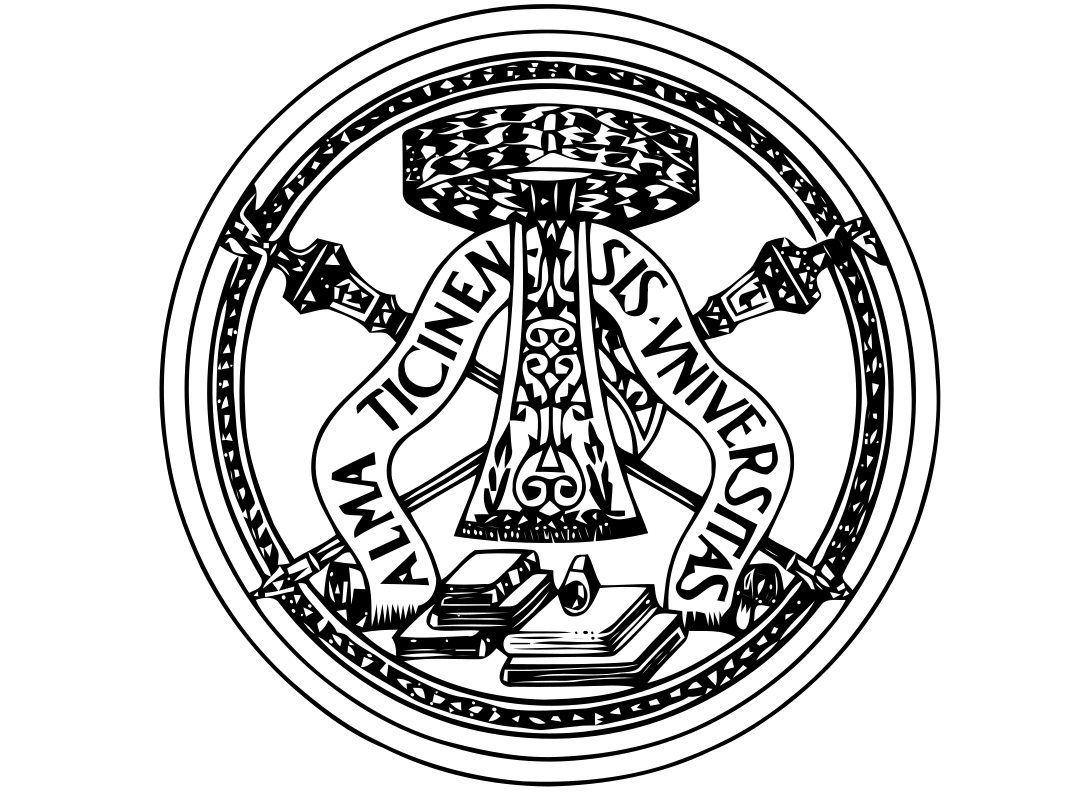
\includegraphics[width=5.5cm]{Risorse/Logo_UNIPV.png}
		\vskip 0.5cm 
		
		\large
			\text {\bf UNIVERSITÀ DEGLI STUDI DI PAVIA}\\
			\text {\bf FACOLTÀ DI INGEGNERIA}\\
			\text {\bf  DIPARTIMENTO DI INGEGNERIA INDUSTRIALE}\\
			\text {\bf E DELL'INFORMAZIONE}\\
			
			\vskip 0.4cm 
		\large \bf
			CORSO DI LAUREA IN INGEGNERIA INFORMATICA
		
		\vskip 3cm
		\Large
			\textbf{Progetto e integrazione del supporto ad Alibaba Cloud su Noovolari Leapp}
		\vskip 4cm
		
		\large
			\begin{flushleft}
			  Relazione discussa in sede di esame finale\\dal candidato Andrea Pusineri
			  \vskip 1cm
			  Tutor universitario: Prof. Luca Lombardi\\
			  Tutor aziendale: Prof. Nicolò Marchesi
			\end{flushleft}
			
			\vfill
			Anno Accademico 2020/2021
	\end{center}
\end{titlepage}

%%%%%%%%%%%%%%%%%%%% Sommario %%%%%%%%%%%%%%%%%%%
\doublespacing
\tableofcontents
\singlespacing
\newpage

%%%%%%%%%%%%%%%%%%%% Introduzione %%%%%%%%%%%%%%%%%%%
\section{Introduzione}
\subsection{beSharp}
beSharp è un'azienda specializzata nell'implementazione e gestione di infrastrutture e servizi Cloud su AWS, con un focus particolare sul design di architetture, sullo sviluppo di applicativi Cloud-native e sull’implementazione di best-practice DevOps.\cite{besharp}

\subsection{Noovolari}
Noovolari è una sezione di beSharp che si concentra sulla ricerca e sviluppo al fine di acquisire conoscenze e portare innovazione all'interno dell'azienda. I progetti realizzati dal team spaziano in diverse aree del Cloud, dalle pipeline adattive per il sequenziamento genomico al backup application-consistent e disaster recovery. Attualmente il team Noovolari è impegnato nello sviluppo di strumenti finalizzati a rendere più efficiente i processi interni dell'azienda.\cite{noovolari}

\subsection{Leapp}
\begin{figure}[ht]
    \centering
    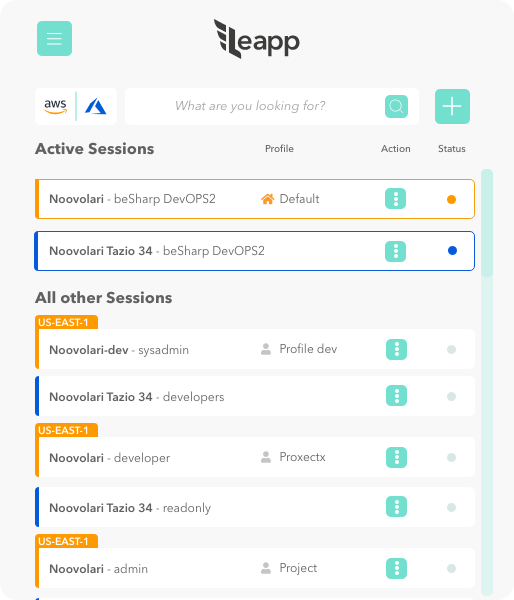
\includegraphics[width=0.5\textwidth]{Risorse/leapp.png}
    \caption{Leapp: sessione d'esempio}
\end{figure}
Leapp è uno strumento che semplifica e rende più sicura la gestione delle credenziali di accesso al Cloud. Si basa sull'idea che salvare le credenziali in chiaro sul computer non sia sicuro in quanto, in caso di compromissione del dispositivo, permettono l'accesso a tutti gli ambienti cloud associati ad esse. Leapp invece salva le credenziali criptate nel keychain del sistema operativo e utilizza per l'autenticazione token temporanei che vengono costantemente rinnovati (di default ogni 20 minuti). È particolarmente utile nel caso si debba gestire un gran numero di credenziali, in quanto automatizza diverse operazioni come il cambio di credenziali attive o il cambio di regione mediante un click sull'interfaccia. Sono inoltre disponibili integrazioni come quella con AWS System Manager, che permette la connessione alle istanze delle macchine virtuali in esecuzione sui server AWS in pochi click. Altre integrazioni sono in fase di sviluppo.\cite{leapp_github}

\subsection{Alibaba Cloud}
Alibaba Cloud, sussidiaria dell'Alibaba Group, conosciuta anche come Aliyun, è il più grosso fornitore di cloud computing cinese, con 23 regioni e 69 availability zones sparse per il mondo, per la maggior parte concentrate in Asia. Offre servizi di Elastic Computing, Networking, CDN, Database, Storage, Security, Analytics e molti altri, tramite una tariffa pay-as-you-go.

\subsection{Progetto}
Leapp attualmente supporta diversi Cloud providers, tra cui Amazon Web Services (AWS), Microsoft Azure e Google Cloud Platform(GCP). Il progetto si è concentrato sull'integrazione del supporto ad Alibaba Cloud in linea con i diversi metodi di autenticazione già presenti e le norme di sicurezza richieste dall'applicazione. Per fare ciò è stata necessaria una prima fase di studio della documentazione del Cloud provider, del linguaggio di programmazione utilizzato nel progetto (Go), della sua architettura e delle sue componenti. Infine, lo sviluppo è avvenuto con un costante confronto con il team responsabile di Leapp, al fine di rispettare la filosofia dell'applicazione.
\newpage

%%%%%%%%%%%%%%%%%%%% Cloud Computing %%%%%%%%%%%%%%%%%%%
\section{Cloud computing}
Il Cloud Computing è un modello che consente l'utilizzo on-demand di un pool condiviso di risorse computazionali programmabili (reti, server, spazio di archiviazione, applicazioni e servizi) che possono essere rese disponibili velocemente e in modo automatizzato, richiedendo un'interazione minima da parte del fornitore.\cite{cloud_computing}

%%%%%%%%%%%%%%%%%%%% Cloud Computing - Caratteristiche%%%%%%%%%%%%%%%%%%%
\subsection{Caratteristiche}
Questo modello è composto da cinque caratteristiche fondamentali:

\begin{itemize}
    \item{\textbf{On-demand self-service}}: i clienti possono acquisire risorse, come tempo di esecuzione o spazio di archiviazione, unilateralmente, quando necessarie e senza intervento manuale da parte del fornitore dei servizi.
    
    \item{\textbf{Broad network access}}: le risorse sono disponibili tramite la rete e accessibili attraverso meccanismi standard che promuovono l'uso di piattaforme client eterogenee.
    
    \item{\textbf{Resource pooling}}: le risorse messe a disposizione dal provider sono raggruppate per servire più clienti contemporaneamente, mediante differenti risorse fisiche e virtuali dinamicamente assegnate in base alla necessità del cliente. Generalmente il cliente non ha controllo e conoscenza della posizione esatta delle risorse assegnate, ma può specificare la posizione desiderata ad un più alto livello di astrazione (paese, datacenter).
    
    \item{\textbf{Rapid elasticity}}: le risorse possono essere allocate e rilasciate in modo elastico, in alcuni casi automaticamente, al fine di scalare proporzionatamente alla richiesta. Per il cliente, le risorse disponibili per l'allocazione spesso sembrano illimitate e accessibili in qualsiasi quantità in ogni momento.
    
    \item{\textbf{Measured service}}: i sistemi Cloud controllano e ottimizzano automaticamente l'uso delle risorse sfruttando una capacità di misurazione ad un certo livello di astrazione del tipo di servizio. Le risorse possono essere monitorate e controllate, fornendo trasparenza sia al provider sia al cliente.\cite{cloud_computing}
\end{itemize}

%%%%%%%%%%%%%%%%%%%% Cloud Computing - Modelli di servizio %%%%%%%%%%%%%%%%%%%
\subsection{Modelli di servizio}
\begin{itemize}
    \item{\textbf{Software  as  a  Service}  (SaaS)}: al cliente viene data la possibilità di usare un'applicazione in esecuzione su un'infrastruttura cloud. Il cliente non ha controllo sull'infrastruttura sottostante all'applicazione, ma ha eventualmente a disposizione un limitato insieme di impostazioni predisposte dall'applicazione.
    
    \item{\textbf{Platform as a Service} (PaaS)}: al cliente viene data la possibilità di rilasciare sull'infrastruttura cloud applicazioni proprie, realizzate mediante tecnologie (linguaggi di programmazione, librerie, servizi) supportate dal fornitore del servizio. Il cliente non ha controllo sull'infrastruttura sottostante all'applicazione, ma ha controllo sull'applicazione e ha la possibilità di configurare impostazioni relative all'ambiente di rilascio.
    
    \item{\textbf{Infrastructure  as  a  Service}  (IaaS)}: al cliente viene data la possibilità di configurare capacità di calcolo, memoria, risorse di rete e altre risorse computazionali fondamentali. Ha anche la possibilità di eseguire software arbitrario, inclusi applicativi e sistemi operativi. Il cliente controlla l'intera infrastruttura cloud, ha il controllo su sistema operativo, capacità di archiviazione, applicazioni eseguite ed eventualmente su un limitato insieme di componenti di rete.\cite{cloud_computing}
\end{itemize}

%%%%%%%%%%%%%%%%%%%% Cloud Computing - Modello multi-cloud %%%%%%%%%%%%%%%%%%%
\subsection{Modello multi-cloud}
Il termine \textit{multi-cloud} fa riferimento all'uso di diversi public cloud service provider per lo storage dei dati virtuali o per l'utilizzo delle risorse di elaborazione. Oltre a offrire alle aziende maggiore flessibilità sulla scelta dei servizi cloud da usare, una strategia multi-cloud riduce la dipendenza da un singolo provider. Le opzioni e le combinazioni multi-cloud offrono diverse possibilità, ad esempio l'infrastruttura di un'azienda può includere l'uso di più provider IaaS per diversi carichi di lavoro e un PaaS pubblico per i test delle nuove applicazioni cloud. Ogni azienda avrà quindi una diversa infrastruttura multi-cloud in base alle diverse esigenze e limitazioni.\cite{multicloud}

%Ho tolto il riferimento all'hybrid cloud che era giusto un accenno. Per quanto riguarda il concetto di cloud agnostic non %sono certo di aver capito cosa intendi, dovrei dire che prevede un'architettura il più possibile indipendente dall'ambiente %cloud, mentre con il multicloud questo non è necessariamente vero in quanto posso semplicemente usare provider diversi per %servizi diversi?

%%%%%%%%%%%%%%%%%%%% Cloud Computing - Modello multi-cloud - Vantaggi %%%%%%%%%%%%%%%%%%%
\subsubsection{Vantaggi}
\begin{itemize}
    \item \textbf{Flessibilità}: optare per diversi servizi cloud offre vantaggi di gran lunga superiori al rischio di eventuali problematiche legate all'uso di vendor diversi. L'adozione di una strategia multi-cloud consente alle aziende di raggiungere gli obiettivi presenti e futuri, senza restare vincolate ai servizi offerti da un singolo provider.
    
    \item \textbf{Velocità}: le aziende di tutto il mondo possono ottenere più rapidamente i servizi scegliendo provider locali di public cloud per le sedi dei loro uffici; più vicino è il data center, minore sarà la latenza. L'utilizzo di un provider locale di public cloud computing diminuisce il tempo di risposta per le attività con priorità elevata.
    
    \item \textbf{Compliance con le normative governative}: alcune aziende possono avere la necessità di utilizzare più provider di storage su cloud per garantire la compliance alle normative governative e alle leggi sulla sovranità dei dati, che prevedono che determinati tipi di dati risiedano nel paese in cui è situata l'azienda.\cite{multicloud}
\end{itemize}
\newpage

%%%%%%%%%%%%%%%%%%% Leapp %%%%%%%%%%%%%%%%%%%
\section{Leapp}
Leapp è un progetto open source nato dalla necessità del team beSharp di gestire la grande mole di strategie di accesso ai diversi ambienti cloud utilizzati ogni giorno. Una best-practice del mondo cloud è appunto la separazione dei workloads, ovvero la divisione su diversi account di permessi di accesso a risorse riservate a scopi differenti, ad esempio gli account per lo sviluppo saranno differenti dagli account di produzione. In questo modo si creano ambienti isolati, senza risorse condivise, rendendo l'accesso più sicuro e riducendo la possibilità di insorgenza di problemi durante lo sviluppo. Uno svantaggio di questo approccio è però l'aumento del numero di strategie di accesso per ogni progetto, che cresce ulteriormente in caso di progetti in ambiente multi-cloud. Leapp si pone l'obbiettivo non solo di semplificare la gestione delle strategie di accesso, ma anche di automatizzare alcuni task. È infatti in sviluppo un sistema di \textit{Actions}, ovvero una sorta di "macro" che permettono di lanciare determinati comandi o eseguire determinate azioni nel contesto di una sessione.

Per quanto riguarda l'implementazione, Leapp è costituita da due componenti principali:
\begin{itemize}
    \item un'interfaccia grafica sviluppata in Typescript, superset di Javascript che introduce la tipizzazione statica, mediante il framework Electron, basato su Node.js e Chromium, che permette di sviluppare applicazioni desktop cross-platform tramite l'utilizzo di tecnologie web come HTML, CSS e Javascript.
    
    \item un demone, scritto in Go, eseguito in background, che svolge automaticamente diverse operazioni di gestione e manutenzione delle credenziali, come il refresh dei token temporanei.
\end{itemize}
È stato scelto di dividere il demone dall'interfaccia,  in modo da avere una conseguente divisione della logica applicativa dall'interfaccia utente. In questo modo è anche possibile comunicare con il demone tramite più e differenti UI (User Interface); oltre alla GUI (Graphical User Interface) già presente, è infatti previsto lo sviluppo di una CLI (Command Line Interface).
\\
Al fine di implementare il supporto ad Alibaba Cloud è stato necessario un focus sul demone, sulla sua architettura, pattern e strutture dati.

%%%%%%%%%%%%%%%%%%% Leapp - Clean Architecture %%%%%%%%%%%%%%%%%%%
\subsection{Clean Architecture}
\begin{figure}[ht]
    \centering
    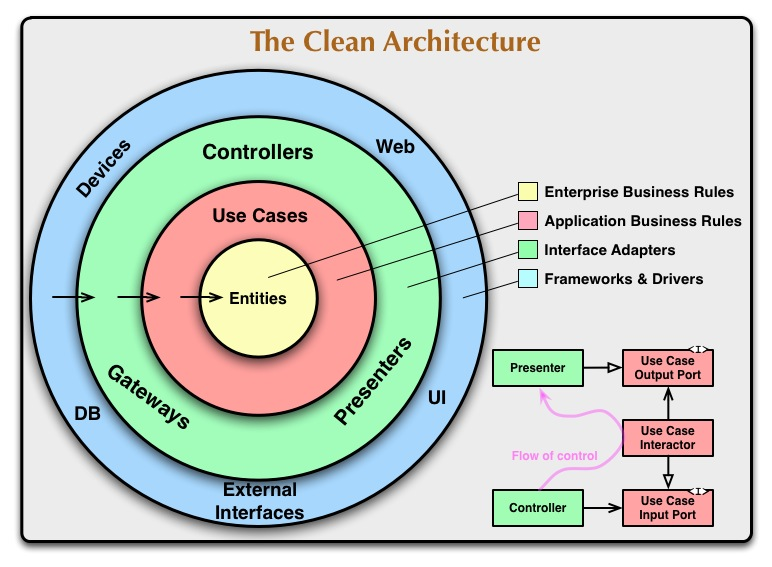
\includegraphics[width=0.8\textwidth]{Risorse/CleanArchitecture.jpg}
    \caption{livelli della Clean Architecture}
\end{figure}
Architettura software che, mediante la divisione in livelli, punta a produrre un sistema:
\begin{itemize}
    \item{\textbf{Indipendente dai framework}}: l'architettura non dipende dall'esistenza di librerie ricche di funzionalità; ciò permette di usare i framework come strumenti anziché dover scrivere il software nei limitati spazi da loro definiti.
    
    \item{\textbf{Testabile}}: la logica di business può essere testata senza la UI, Database, Web Server o altri elementi esterni.
    
    \item{\textbf{Indipendente dalla UI}}: la UI può essere sostituita facilmente, passando ad esempio da una Web UI a una CLI, senza modificare la logica di business.
    
    \item{\textbf{Indipendente dal database}}: il database può essere sostituito facilmente, in quanto la logica di business non è legata ad esso.
    
    \item{\textbf{Indipendente da fattori esterni}}: la logica di business non conosce nulla sui livelli esterni.\cite{clean_architecture}
\end{itemize}

%%%%%%%%%%%%%%%%%%% Leapp - Clean Architecture - Dependecy Rule %%%%%%%%%%%%%%%%%%%
\subsubsection{Dependency rule}
Ogni cerchio del grafico rappresenta una diversa area del software, i cerchi man mano più interni diventano di livello sempre più alto.
Secondo questa regola le dipendenze possono puntare solo verso l'interno, nulla dei cerchi più interni può assumere nulla sui più esterni, nulla dei cerchi esterni deve influenzare quelli interni.
\begin{itemize}
    \item{\textbf{Entities}}: Le entità incapsulano la logica di business, un'entità può essere nella forma di un oggetto con i propri metodi o una struttura dati con le proprie funzioni. Nessuna modifica dell'implementazione deve richiedere modifiche in questo livello.

    \item{\textbf{Use Cases}}: Questo livello contiene la logica di business specifica dell'applicazione, incapsula e implementa tutti i casi d'uso del sistema. Questi casi d'uso gestitscono il flusso di dati da e verso le entità. I cambiamenti in questo livello non devono influenzare le entità, allo stesso modo cambiamenti di interfaccia utente, database o altri elementi esterni non devono influenzare questo livello. Ciò che richiede modifiche in questo livello sono i cambiamenti nelle funzionalità del sistema.

    \item{\textbf{Interface Adapters}}: Livello costituito da un insieme di adattatori che convertono i dati dal formato più conveniente per le entità e i casi d'uso, al formato più conveniente per entità esterne, come un database o un'applicazione web e viceversa.

    \item{\textbf{Frameworks e drivers}}: È il livello più esterno, solitamente composto da database e web frameworks. Generalmente questo livello non richiede molto codice all'infuori di quello necessario alla comunicazione con il livello interno.\cite{clean_architecture}
\end{itemize}

%%%%%%%%%%%%%%%%%%% Leapp - Clean Architecture - Passaggio di dati tra livelli%%%%%%%%%%%%%%%%%%%
\subsubsection{Passaggio di dati tra livelli}
I dati scambiati tra i livelli sono semplici strutture dati, l'importante è che siano semplici ed isolate. Non devono essere passate strutture di livelli più bassi come entità o di livelli più alti come entrate di database. Passare l'entrata di un database ad uno strato inferiore violerebbe la Dependecy Rule, richiedendo al livello interno di avere informazioni su uno più esterno.\cite{clean_architecture}

%%%%%%%%%%%%%%%%%%% Leapp - Clean Architecture - Implementazione in Go %%%%%%%%%%%%%%%%%%%
\subsubsection{Implementazione in Go}
\begin{table}[ht]
\small
\begin{tabular}{lccr} %lcr indica dove la prima,seconda e terza riga si devono allineare. lef centro e right
    \toprule
    Infrastructure & Interfaces & Use Cases & Domain \\
    \midrule
    application-agnostic & application-specific & application-specific & application-agnostic\\
    business-agnostic & business-agnostic & business-specific & business-specific\\
    \bottomrule
\end{tabular}
\vskip 0.2cm
\caption{Schema di implementazione}
\end{table}

L'implementazione dei concetti espressi dalla Clean Architecture varia a seconda dei tipi di strutture dati e degli strumenti messi a disposizione dal linguaggio di programmazione utilizzato.\\

\textbf{Dependecy Rule}: in un livello interno viene definita un'interfaccia astratta che non fa riferimento a nessun livello più esterno, mentre la sua implementazione è definita in un livello più esterno. L'implementazione è poi \textit{iniettata} nel livello che deve utilizzarla.\\
La \textit{Dependency Injection} è l'idea che i componenti del sistema (strutture in Go) debbano ricevere le dipendenze alla creazione. Supponendo di avere una struttura Server che richiede una struttura Config, un esempio di Dependency Injection è:
\begin{lstlisting}[style=customgo, caption=esempio di Dependency Injection, captionpos=b]
type Server struct {
    config *Config
}

func New() *Server {
    return &Server{
        config: buildConfig(),
    }
}
\end{lstlisting}
In questo modo il chiamante non necessita di sapere che Server richiede Config.\cite{dep_inj}\cite{clean_implementation}\\
Per ogni componente di ogni livello è necessario porsi 3 domande:
\begin{itemize}
    \item in che livello viene utilizzato?
        
    \item in che livello è presente la sua interfaccia?
        
    \item in che livello è presente la sua implementazione?
\end{itemize}

\textbf{Pattern Repository}: pattern che permette di disaccoppiare la logica applicativa dalla logica del database, in modo da permettere di sostituirlo facilmente ed evitare di rimanerne vincolati. Si basa sull'idea di astrarre l'implementazione del database definendo le interazioni con esso tramite un'interfaccia che deve poter essere usata con ogni tipo di database implementato, di conseguenza deve essere priva di dettagli implementativi specifici. Questo metodo permette anche di posticipare la scelta del database da utilizzare, dando la precedenza allo sviluppo del Domain, in base al quale verrà poi effettuata la scelta mgliore.\cite{go_with_domain}

\begin{lstlisting}[style=customgo, caption=esempio di implementazione del pattern Repository, captionpos=b]
package interfaces

type DbHandler interface {
    Execute(statement string)
    Query(statement string) Row
}|\Suppressnumber|

|\Reactivatenumber{1}|
package infrastructure

type SqliteHandler struct {
    Conn *sql.DB
}

func (handler *SqliteHandler) Execute(statement string) {
    handler.Conn.Exec(statement)
}

func (handler *SqliteHandler) Query(statement string) interfaces.Row {
    rows, err := handler.Conn.Query(statement)
    if err != nil {
    	fmt.Println(err)
	    return new(SqliteRow)
	}
    row := new(SqliteRow)
    row.Rows = rows
    return row
}
\end{lstlisting}

\newpage
%%%%%%%%%%%%%%%%%%% Esperienza di tirocinio %%%%%%%%%%%%%%%%%%%
\section{Esperienza di tirocinio}
La prima parte del tirocinio è stata dedicata allo studio della documentazione di Alibaba Cloud, in modo da acquisire le conoscenze necessarie per poter progettare l'integrazione con il Cloud provider. In particolare, ai fini del progetto, è particolarmente interessante il servizio Alibaba RAM.
%%%%%%%%%%%%%%%%%%% Esperienza di tirocinio - Alibaba RAM %%%%%%%%%%%%%%%%%%%
\subsection{Alibaba RAM}
Alibaba Cloud Resource Access Management (RAM) è uno dei tanti servizi offerti da Alibaba Cloud. Questo servizio permette di gestire le identità di accesso presenti sotto un account Alibaba Cloud. Tramite RAM è quindi possibile creare, modificare ed eliminare utenti, ruoli e permessi.\cite{alibaba_ram}

%%%%%%%%%%%%%%%%%%% Esperienza di tirocinio - Alibaba RAM - Utenti %%%%%%%%%%%%%%%%%%%
\subsubsection{Utenti}
Un utente RAM corrisponde ad un'identità composta da un ID e delle credenziali. Un account Alibaba Cloud può avere più utenti RAM che rappresentano dipendenti, sistemi o applicazioni all'interno di un'organizzazione. Gli utenti RAM non posseggono risorse, le spese dovute alle loro azioni sono addebitate all'account Alibaba Cloud corrispondente, i singoli utenti non ricevono conti e non possono eseguire pagamenti. Le organizzazioni possono utilizzare RAM per gestire i permessi degli utenti e le loro azioni sulle risorse.\cite{alibaba_users}
\begin{figure}[ht]
    \centering
    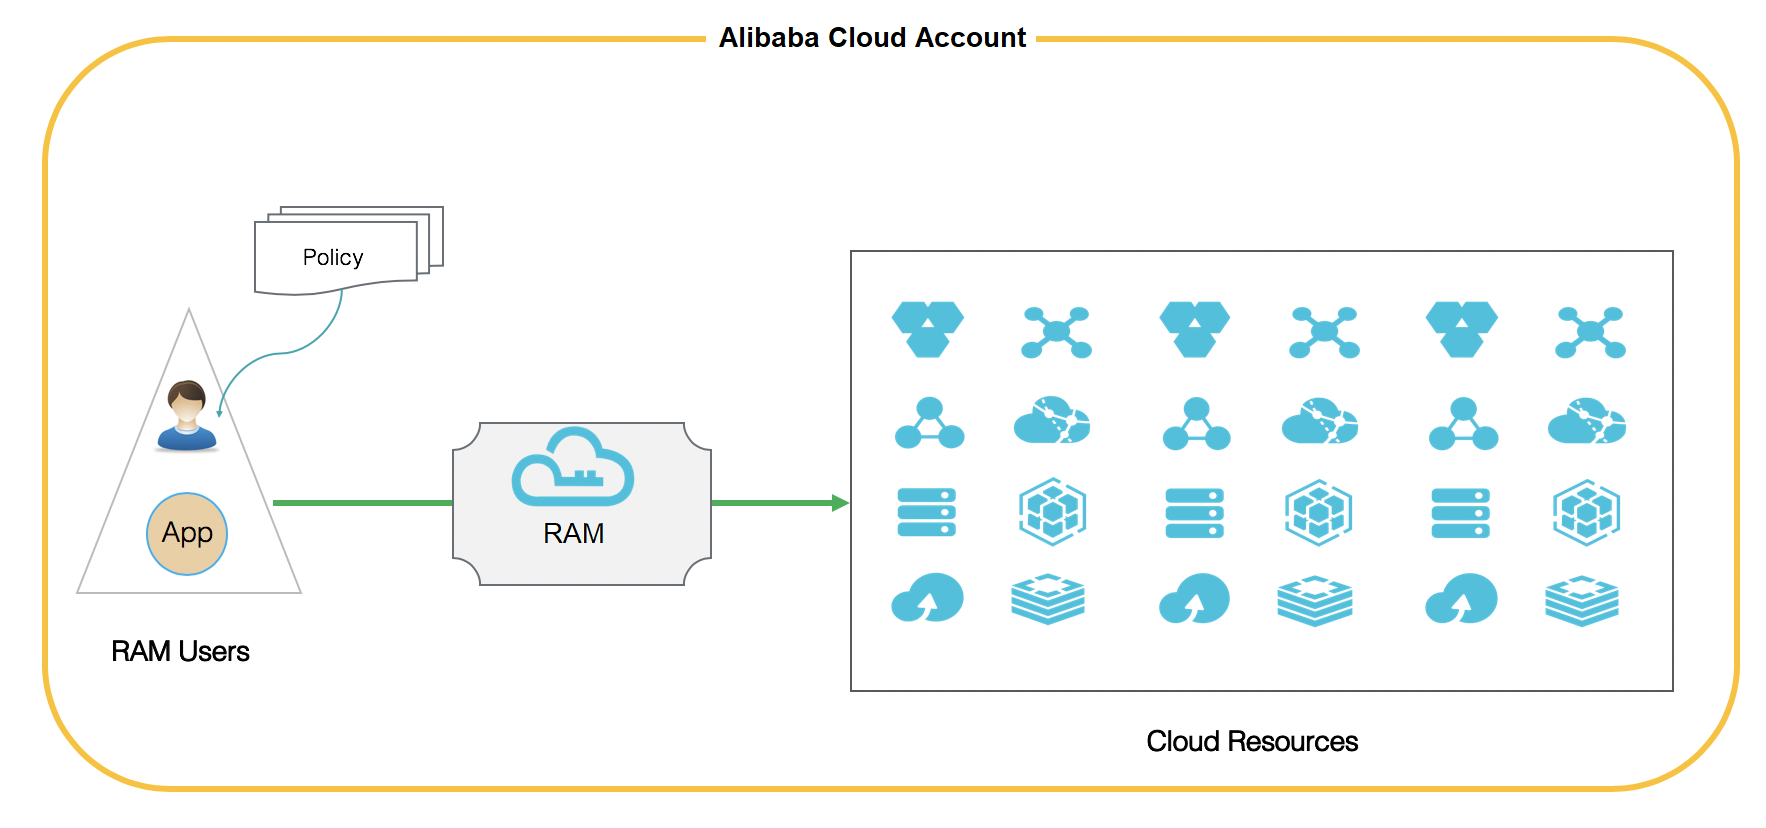
\includegraphics[width=0.9\textwidth]{Risorse/alibaba_user_permission.png}
    \caption{Utente RAM}
\end{figure}\\

%%%%%%%%%%%%%%%%%%% Esperienza di tirocinio - Alibaba RAM - Ruoli %%%%%%%%%%%%%%%%%%%
\subsubsection{Ruoli}
Un ruolo RAM è un'identità virtuale a cui è associato un insieme di permessi definiti tramite policies. A differenza dell'utente RAM non possiede una password di accesso o delle AccessKey. Un ruolo può essere utilizzato solo dopo essere stato "assunto" da un'entità (utente o servizio), ad esempio un utente con insufficienti permessi per eseguire un'operazione può "assumere" temporaneamente un ruolo con i permessi necessari, purché ne sia abilitato. In questo modo i ruoli permettono di dare accesso temporaneo a un insieme di permessi ad agenti esterni come consulenti o fornitori, senza i ruoli sarebbe stato necessario creare utenti ad-hoc coi permessi necessari e da eliminare in seguito.\\
Ogni ruolo, come anche le istanze dei vari servizi, è definito universalmente da un identificatore univoco detto Alibaba Cloud Resource Name (ARN). L'ARN di un ruolo è espresso come:
\vskip 0.3cm
\begin{lstlisting}
   acs:ram::1234567890123456:role/samplerole
\end{lstlisting}
\vskip 0.3cm
L'ARN di ogni ruolo RAM è assegnato durante la creazione.\cite{alibaba_roles}
\begin{figure}[ht]
    \centering
    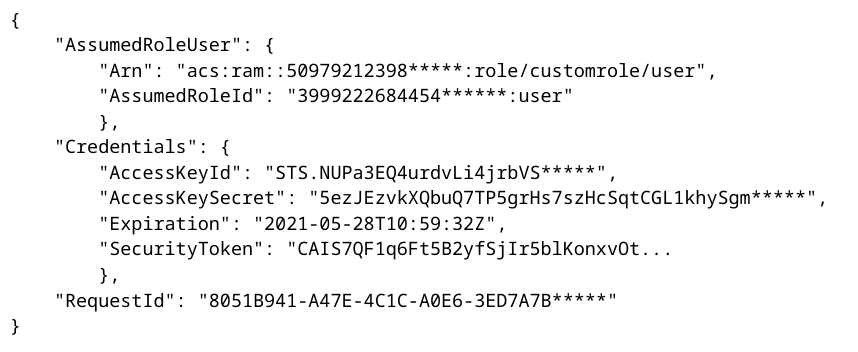
\includegraphics[width=0.9\textwidth]{Risorse/role.png}
    \caption{Esempio di output della chiamata AssumeRole}
\end{figure}\\

%%%%%%%%%%%%%%%%%%% Esperienza di tirocinio - Alibaba RAM - Metodi di autenticazione %%%%%%%%%%%%%%%%%%%
\subsubsection{Metodi di autenticazione}
Alibaba Cloud supporta i seguenti metodi di autenticazione:
\begin{itemize}
    \item{\textbf{AccessKey pair}}: è il metodo più semplice di autenticazione. Ad ogni utente, durante la sua creazione, è automaticamente assegnata una coppia di chiavi alfanumeriche, un \textit{AccessKey ID} e un \textit{AccessKey Secret}, mediante cui può effettuare l'accesso alla console o fare chiamate alle API. Eventualmente, per rendere l'accesso più sicuro, può essere aggiunto un sistema di autenticazione multifattore, che viene però utilizzato solo durante l'autenticazione per l'accesso alla Console, non per l'uso delle API o dell'SDK.\cite{alibaba_ak}
    
    \item{\textbf{StsToken}}: un StsToken è una stringa che permette l'assunzione di un ruolo RAM per una limitata finestra di tempo. Questa soluzione offre vantaggi in termini di sicurezza, in quanto permette di fornire l'accesso temporaneo a un ruolo, e di conseguenza a un preciso insieme di permessi. Nel caso si voglia permettere l'assunzione di un ruolo ad un utente RAM esterno all'organizzazione, è necessario specificare l'ID di tale utente in fase di creazione del ruolo.\cite{alibaba_access}
    
    \item{\textbf{RamRoleArn}}: come l'StsToken permette l'assunzione di un ruolo RAM, ma in questo caso il token è costantemente rinnovato in modo automatico. È una soluzione più comoda nel caso il ruolo RAM debba essere assunto da un utente RAM interno all'organizzazione.\cite{alibaba_access}
    
    \item{\textbf{EcsRamRole}}: questo metodo di autenticazione prende il nome da Elastic Compute Service (ECS), un servizio di tipo IaaS che consente di creare macchine virtuali su Alibaba Cloud. Permette ad un servizio di Alibaba Cloud di assumere un ruolo RAM al fine di ottenere i permessi per eseguire determinate operazioni, specificate in un insieme di policies associate ad esso.\cite{alibaba_ecsrole}
    
    \item{\textbf{Single Sign-On} (SSO)}: Alibaba Cloud supporta il protocollo SAML2.0 per l'autenticazione tramite federazione, permettendo la comunicazione tra \textit{Service Provider} (SP) e \textit{Identity Provider} (IdP). Un IdP è un'entità che crea e gestisce le identità degli utenti e fornisce servizi di autenticazione all'interno di una federazione, mentre un SP è un'entità che fornisce dei servizi.
    In particolare ci sono due tipi di accesso SSO: User-Based e Role-Based, che definiscono rispettivamente l'utente RAM o il ruolo RAM assegnato in seguito all'autenticazione. I vantaggi di un approccio di questo tipo sono la semplificazione del controllo degli utenti e la riduzione del numero di password da gestire, in quanto ogni utente fisico ha associata una sola coppia di credenziali. È però necessaria una configurazione sia lato IdP che lato SP.\cite{alibaba_sso}
\end{itemize}

%%%%%%%%%%%%%%%%%%% Esperienza di tirocinio - Alibaba RAM - SAML2.0 %%%%%%%%%%%%%%%%%%%
\subsubsection{SAML2.0}
Il Security Assertion Markup 2.0 è una versione dello standard SAML per lo scambio di dati di autenticazione e autorizzazoni tra più domini differenti. È un protocollo basato sullo scambio di documenti XML tra più autorità SAML. I documenti in questione contengono \textit{Asserzioni} tramite cui vengono passate informazioni riguardo un utente, detto \textit{Principal}. Il protocollo permette quindi l'uso di web-based, cross-domain Single Sign-On (SSO), che consentono di ridurre l'overhead amministrativo dovuto alla distribuzione di credenziali agli utenti.

\begin{figure}[ht]
    \centering
    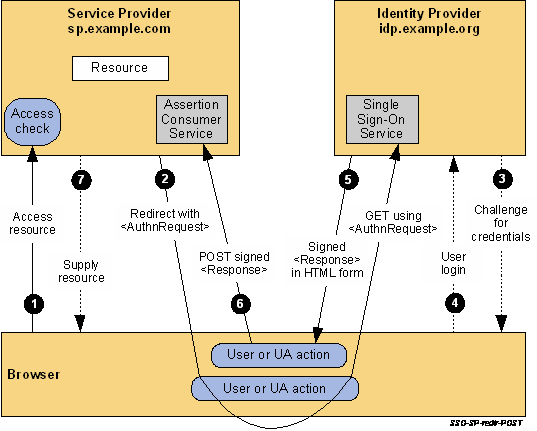
\includegraphics[width=0.7\textwidth]{Risorse/saml.png}
    \caption{Esempio di SP-Initiated SSO}
\end{figure}

Come evidenziato nella grafico, l'autenticazione federata tramite SAML2.0 è composta di diversi passaggi:
\begin{enumerate}
    \item L'utente richiede al SP l'accesso alla risorsa, ma non possiede una sessione valida.
    
    \item Il SP invia un redirect HTTP come risposta al browser (tramite uno status HTTP 302 o 303) contenente un header Location con URI di destinazione diretto al servizio di Sign-On dell' IdP. Il redirect contiene inoltre un messaggio <AuthnRequest> codificato in base64, presente nell'URL come parametro e chiamato \textit{SAMLRequest}.
    
    \item Il servizio di SSO determina se l'utente possiede già una sessione attiva e se ha i permessi per accedere alla risorsa richiesta al SP. Se l'utente non possiede sessioni attive, l'IdP richiede all'utente le credenziali di accesso.
    
    \item L'utente fornisce delle credenziali valide e l'IdP crea una sessione per l'utente.
    
    \item L'IdP genera un'asserzione SAML che rappresenta la sessione dell'utente, che viene firmata digitalmente e inserita in un messaggio <Response>. Il messaggio viene a sua volta inserito in una FORM HTML nascosta, chiamata \textit{SAMLResponse}. 
    
    \item Il browser esegue automaticamente una richiesta HTTP POST contenente la form al SP. Il SP ottiene la form ed estrae il messaggio <Response>, valida la firma digitale sull'asserzione e invia un redirect HTTP diretto alla risorsa inizialmente richiesta al browser.
    
    \item Viene infine effettuato un controllo per verificare se l'utente ha i permessi per richiedere la risorsa che, in caso positivo, gli viene fornita.\cite{saml}
\end{enumerate}


\subsection{Struttura progetto}
Poiché il progetto era già in fase di sviluppo, prima dell'implementazione del supporto per Alibaba Cloud, è stato necessario studiare il codice già presente per poterne sfruttare funzioni e strutture dati, al fine di evitare il più possibile di creare codice duplicato. In Figura \ref{fig:strut} è riportato un diagramma estremamente semplificato delle interazioni tra i vari livelli del programma.\\\\
\begin{figure}[ht]
    \centering
    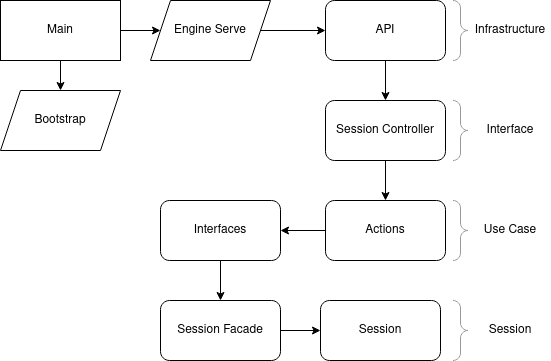
\includegraphics[width=0.9\textwidth]{Risorse/PianoForge.png}
    \caption{Struttura semplificata del demone}
    \label{fig:strut}
\end{figure}
Appena avviato il programma, il file \textit{main.go} esegue delle operazioni di inizializzazione, di cui le più importanti sono:
\begin{itemize}
    \item \textit{Bootstrap}: fase in cui vengono letti i dati persistenti. In particolare viene usato il file \textit{.Leapp.json}, opportunamente criptato, per salvare i dati relativi alle sessioni presenti nel programma.
    \item \textit{Engine Serve}: fase in cui il server viene messo in ascolto sulla porta designata, mettendo a disposizione le API.
\end{itemize}
Nel livello più esterno, l'Infrastruttura, sono presenti delle API REST implementate tramite il framework \textit{gin}\cite{gin}. \\
Ricevuta la richiesta di un client, a seconda della route utilizzata, viene richiamata la funzione associata in un \textit{Session Controller}, presente nel livello dell'Interfaccia. Sono presenti diversi Session Controller, suddivisi per ogni Cloud provider e metodo di autenticazione supportato, ognuno di essi mette a disposizione classiche funzioni di tipo CRUD\cite{crud} e alcune funzioni relative al dominio dell'applicazione.\\
I Session Controller interpretano la richiesta e passano i parametri alle \textit{Actions}, presenti nel livello sottostante, quello dei Casi d'Uso. Anche in questo caso sono presenti Actions per ogni Cloud provider e metodo di autenticazione supportato. Queste svolgono effettivamente la richiesta, manipolando le strutture dati tramite i metodi a loro associati mediante l'interazione con interfacce utilizzate per il disaccoppiamento e per rendere più semplice il testing delle funzionalità.\\
Nel livello più interno sono infine presenti le \textit{Session}, strutture dati corrispondenti alle sessioni di ogni Cloud provider supportato. Ognuna di esse ha associata una \textit{Session façade} che ne espone i metodi.

\subsection{Sviluppo}
Per poter integrare il supporto ad Alibaba Cloud è stato necessario creare ognuna delle componenti del paragrafo precedente per il nuovo provider. Il lavoro è stato suddiviso in base ai metodi di autenticazione supportati da Leapp.

\subsubsection{RAM User Access}
Questo metodo di autenticazione si riferisce al classico Utente RAM con AccessKey pair.

Relativamente al livello più esterno, quello dell'Infrastruttura, è stato sufficiente aggiungere delle nuove route alle API, operazione semplificata dall'utilizzo del framework gin.
\begin{lstlisting}[style=customgo, caption=engine.go (righe 53-92), captionpos=b, firstnumber=53]
func initializeRoutes(ginEngine *gin.Engine) {
	v1 := ginEngine.Group("/api/v1") { |\Suppressnumber|
...|\Reactivatenumber{85}|
		v1.GET("/alibaba/ram-user-sessions/:id", controller.GetAlibabaRamUserSessionController)
		v1.POST("/alibaba/ram-user-sessions/", controller.CreateAlibabaRamUserSessionController)
		v1.PUT("/alibaba/ram-user-sessions/:id", controller.UpdateAlibabaRamUserSessionController)
		v1.DELETE("/alibaba/ram-user-sessions/:id", controller.DeleteAlibabaRamUserSessionController)
		v1.POST("/alibaba/ram-user-sessions/:id/start", controller.StartAlibabaRamUserSessionController)
		v1.POST("/alibaba/ram-user-sessions/:id/stop", controller.StopAlibabaRamUserSessionController)
	}
}
\end{lstlisting}
Ad ogni route è associata una funzione del Session Controller, in linea di massima tutte seguono gli stessi passi:
\begin{enumerate}
 \item Interpretare la richiesta del client (ottenuta sotto forma di DTO\footnote{Data Transfer Object, un oggetto software che incapsula dei dati al fine di trasportarli tra diversi sottosistemi.}).
 \item Richiamare la funzione della Action associata, passandole i parametri estratti dalla richiesta.
 \item Preparare una risposta e inviarla al client.
\end{enumerate}

Le Actions, attraverso le Session façade, manipolano direttamente i dati del dominio, ad esempio la funzione di creazione di una nuova Session (riportata nel Listato successivo) esegue dei controlli sui dati inseriti, come la validità della Region, imposta i campi della Session e salva nel Keychain le credenziali.

\begin{lstlisting}[style=customgo, caption=alibaba\_ram\_user\_session\_actions.go (righe 11-58), captionpos=b, firstnumber=11]
type AlibabaRamUserSessionActions struct {
	Environment                  Environment
	Keychain                     Keychain
	NamedProfilesActions         NamedProfilesActionsInterface
	AlibabaRamUserSessionsFacade AlibabaRamUserSessionsFacade
}

func (actions *AlibabaRamUserSessionActions) Create(alias string, alibabaAccessKeyId string, alibabaSecretAccessKey string, regionName string, profileName string) error {

	namedProfile, err := actions.NamedProfilesActions.GetOrCreateNamedProfile(profileName)
	if err != nil {
		return err
	}

	isRegionValid := region.IsAlibabaRegionValid(regionName)
	if !isRegionValid {
		return http_error.NewUnprocessableEntityError(fmt.Errorf("Region " + regionName + " not valid"))
	}

	alibabaRamUserAccount := session.AlibabaRamUserAccount{
		Region:         regionName,
		NamedProfileId: namedProfile.Id,
	}

	sess := session.AlibabaRamUserSession{
		Id:      actions.Environment.GenerateUuid(),
		Alias:   alias,
		Status:  session.NotActive,
		Account: &alibabaRamUserAccount,
	}

	err = actions.AlibabaRamUserSessionsFacade.AddSession(sess)
	if err != nil {
		return err
	}

	err = actions.Keychain.SetSecret(alibabaAccessKeyId, sess.Id+constant.PlainAlibabaKeyIdSuffix)
	if err != nil {
		return http_error.NewInternalServerError(err)
	}

	err = actions.Keychain.SetSecret(alibabaSecretAccessKey, sess.Id+constant.PlainAlibabaSecretAccessKeySuffix)
	if err != nil {
		return http_error.NewInternalServerError(err)
	}

	return nil
}
\end{lstlisting}

La struttura \textit{AlibabaRamUserSessionActions} possiede come attributi diversi elementi, definiti tramite interfacce, i cui metodi vengono utilizzati all'interno della classe. Questa strategia è preferita a una chiamata diretta ai metodi, al fine di permettere un testing più semplice e completo. In questo modo è possibile realizzare dei mock, ovvero degli elementi che simulano il comportamento di dipendenze al fine di testare il comportamento di un oggetto, iniettandoli al posto delle dipendenze reali.\\
Uno degli attributi della struttura è la Session façade, ovvero la componente che effettivamente manipola i dati nella Session; in seguito alla chiamata ad AddSession() della riga 42, verrà chiamato il seguente metodo:

\begin{lstlisting}[style=customgo, caption=alibaba\_ram\_user\_session\_facade.go (righe 64-98), captionpos=b, firstnumber=64]
func (fac *AlibabaRamUserSessionsFacade) AddSession(alibabaRamUserSession AlibabaRamUserSession) error {
	alibabaRamUserSessionsLock.Lock()
	defer alibabaRamUserSessionsLock.Unlock()

	oldAlibabaRamUserSessions := fac.GetSessions()
	newAlibabaRamUserSessions := make([]AlibabaRamUserSession, 0)

	for i := range oldAlibabaRamUserSessions {
		newAlibabaRamUserSession := oldAlibabaRamUserSessions[i]
		newAlibabaRamUserSessionAccount := *oldAlibabaRamUserSessions[i].Account
		newAlibabaRamUserSession.Account = &newAlibabaRamUserSessionAccount
		newAlibabaRamUserSessions = append(newAlibabaRamUserSessions, newAlibabaRamUserSession)
	}

	for _, sess := range newAlibabaRamUserSessions {
		if alibabaRamUserSession.Id == sess.Id {
			return http_error.NewConflictError(fmt.Errorf("a AlibabaRamUserSession with id " + alibabaRamUserSession.Id +
				" is already present"))
		}

		if alibabaRamUserSession.Alias == sess.Alias {
			return http_error.NewUnprocessableEntityError(fmt.Errorf("a session with the same alias " +
				"is already present"))
		}
	}

	newAlibabaRamUserSessions = append(newAlibabaRamUserSessions, alibabaRamUserSession)

	err := fac.updateState(newAlibabaRamUserSessions)
	if err != nil {
		return err
	}

	return nil
}
\end{lstlisting}

Per quanto riguarda la Session, è stata sufficiente una semplice struttura contenete alcuni parametri, tra cui i principali:
\begin{itemize}
 \item \textbf{Id}: un identificatore univoco della sessione.
 \item \textbf{Status}: lo stato corrente della sessione, che può essere Active, Inactive o Pending.
 \item \textbf{Region}: la regione in cui si trova la sessione.
\end{itemize}

\begin{lstlisting}[style=customgo, caption=alibaba\_ram\_user\_session.go (righe 9-19), captionpos=b, firstnumber=9]
type AlibabaRamUserSession struct {
	Id      string
	Alias   string
	Status  Status
	Account *AlibabaRamUserAccount
}

type AlibabaRamUserAccount struct {
	Region         string
	NamedProfileId string
}
\end{lstlisting}

\subsubsection{RAM Role Federated Access}
Questo metodo di autenticazione si riferisce all'accesso tramite SSO Role-Based.

La differenza fondamentale tra l'implementazione di questo metodo di autenticazione ed il precedente è il fatto che le credenziali per l'accesso al Cloud non sono più note a priori, ma per ottenerle è necessario interagire con l'SDK (Software Development Kit) messo a disposizione da Alibaba Cloud. In particolare viene chiamato il metodo \textit{AssumeRoleWithSAML()} dell'SDK nella funzione \textit{SAMLAuth()}, presente nel livello dei Casi d'Uso e riportata in seguito:

\begin{lstlisting}[style=customgo, caption=alibaba\_ram\_role\_federated\_session\_actions.go (righe 20-36), captionpos=b, firstnumber=20]
func SAMLAuth(region string, idpArn string, roleArn string, assertion string) (key string, secret string, token string, err error) {
	client, _ := sts.NewClientWithAccessKey(region, "", "")

	request := sts.CreateAssumeRoleWithSAMLRequest()
	request.Scheme = "https"
	request.SAMLProviderArn = idpArn
	request.RoleArn = roleArn
	request.SAMLAssertion = assertion
	response, err := client.AssumeRoleWithSAML(request)
	if err != nil {
		return "", "", "", err
	}
	key = response.Credentials.AccessKeyId
	secret = response.Credentials.AccessKeySecret
	token = response.Credentials.SecurityToken
	return
}
\end{lstlisting}
Nel codice le funzioni dell'SDK fanno riferimento alla libreria \textit{github.com/aliyun/alibaba-cloud-sdk-go/services/sts}. È inoltre importante menzionare che la creazione del client tramite la funzione \textit{NewClientWithAccessKey()} senza credenziali è un workaround dovuto al fatto che la funzione più adatta \textit{NewClient()}, seppur presente nell'SDK, non è ancora stata effettivamente implementata ed il tentativo di utilizzarla porta alla terminazione forzata del programma con un errore. La soluzione riportata è comunque perfettamente funzionante, ma è da intendersi come una soluzione temporanea in attesa del completamento dell'SDK.\\

La Session rispetto al caso precedente è leggermente più complessa in quanto il metodo di autenticazione richiede più parametri.
\begin{lstlisting}[style=customgo, caption=alibaba\_ram\_role\_federated\_session.go (righe 14-35), captionpos=b, firstnumber=14]
type AlibabaRamRoleFederatedSession struct {
	Id        string
	Status    Status
	StartTime string
	Account   *AlibabaRamRoleFederatedAccount
	Profile   string
}

type AlibabaRamRoleFederatedAccount struct {
	AccountNumber string
	Name          string
	Role          *AlibabaRamRole
	IdpArn        string
	Region        string
	/*SsoUrl        string*/
	NamedProfileId string
}

type AlibabaRamRole struct {
	Name string
	Arn  string
}
\end{lstlisting}
Rispetto alla Session del Plain sono presenti in più i parametri:
\begin{itemize}
    \item \textbf{Role}: puntatore che fa riferimento ad una struttura \textit{AlibabaRamRole} contenente il nome e l'ARN del ruolo da assumere.
    \item \textbf{IdpArn}: l'ARN dell'Identity Provider tramite cui viene eseguita l'autenticazione.
\end{itemize}

\subsubsection{RAM Role Chained Access}
Questo metodo di autenticazione si riferisce all'assunzione di un ruolo da parte di un utente di un account Alibaba Cloud differente. Di conseguenza per effettuare questo tipo di autenticazione è necessario avere già un accesso con una delle altre due modalità a cui sarà legato il ruolo, ciò si rispecchia nell'implementazione della Session:
\begin{lstlisting}[style=customgo, caption=alibaba\_ram\_role\_chained\_session.go (righe 9-29), captionpos=b, firstnumber=9]
type AlibabaRamRoleChainedSession struct {
	Id            string
	Status        Status
	StartTime     string
	ParentId      string
	ParentType    string
	Account       *AlibabaRamRoleChainedAccount
	Profile       string
}

type AlibabaRamRoleChainedAccount struct {
	AccountNumber string
	Name          string
	Role          *AlibabaRamRole
	Region        string
}
\end{lstlisting}
La differenza principale rispetto alla Session del Federated è l'introduzione degli attributi:
\begin{itemize}
    \item \textbf{ParentId}: fa riferimento all' ID dell'account che assume il ruolo.
    \item \textbf{ParentType}: specifica tramite una stringa il tipo dell'account che assume il ruolo.
\end{itemize}
Questi attributi sono necessari a specificare a quale sessione tra quelle già presenti farà riferimento la chiamata all'SDK per l'assunzione del ruolo. Il problema però è che il ruolo può essere assunto da più tipi di sessione, ma, non potendo sapere quale dei tipi lo assume, non è possibile chiamarne i metodi. È stata quindi realizzata un'interfaccia \textit{ParentSession} che definisce le firme dei metodi utili all'acquisizione delle informazioni necessarie; i tipi di sessione dovranno poi implementare questi metodi per poter essere utilizzati come ParentSession. Così facendo non è necessario conoscere il tipo di sessione legata al ruolo ed è facile ottenerne Id e tipo.
\begin{lstlisting}[style=customgo, caption=parent\_interface.go (righe 3-6), captionpos=b, firstnumber=3]
type ParentSession interface {
	GetId() string
	GetTypeString() string
}
\end{lstlisting}

L'implementazione dello Use Case è molto simile alla precedente, è invece modificata l'interazione con l'SDK, che in questo caso viene fatta attraverso la chiamata \textit{CreateAssumeRoleRequest()}
\begin{lstlisting}[style=customgo, caption=alibaba\_ram\_role\_chained\_session\_actions.go (righe 208-212), captionpos=b, firstnumber=208]
request := sts.CreateAssumeRoleRequest()
	request.Scheme = "https"
	request.RoleArn = sess.Account.Role.Arn
	request.RoleSessionName = "leapp"
	response, err := client.AssumeRole(request)
\end{lstlisting}

\newpage

\section{Conclusioni}
Terminato lo sviluppo dell'estensione di Leapp ad Alibaba Cloud, il team di beSharp è in grado di interagire con il nuovo provider con la stessa semplicità con la quale utilizzava Amazon Web Services, Microsoft Azure o Google Cloud Platform. Inoltre, l'aver sviluppato il supporto ad Alibaba Cloud in modo quanto più possibile in linea con i servizi già presenti nell'applicazione, ha permesso al team di conservare inalterato il proprio metodo di lavoro, portandolo quindi a poter interagire con un nuovo provider senza soluzione di continuità.
\newpage
\printbibliography
\end{document}
